\chapter{Private Value Auctions}

Under the private value setting, we have $n$ bidders and a single object. Each bidder draws a value $X_i\sim F$ independently. Only bidder $i$ knows their own value $X_i = x_i$, and the distribution $F$ is common knowledge. Each bidder submits a bid $b_i$ to the auctioneer, and the auctioneer determines the winner and the price to be paid based on the bids.

\section{Second Price Sealed Bid Auction (SPA)}

In a second price sealed bid auction, each bidder submits a bid without knowing the bids of others. The highest bidder wins the item, but pays the second-highest bid.

\clmp{}{
  It is a weakly dominant strategy for each bidder to bid their true value in a SPA, i.e., $b_i = x_i$.
}{
Graphical proof:

Suppose bidder 1 has value $x_1$. We want to show that bidding $b_1 = x_1$ is a weakly dominant strategy for bidder 1. Let $x_{-1}$ be the highest competing bid among the other bidders. The profit for bidder 1 is given by:
\[
\pi_1(b_1, x_{-1}) = \begin{cases}
x_1 - x_{-1} & \text{if } b_1 > x_{-1},\\
0 & \text{if } b_1 < x_{-1}.\\
\end{cases}
\]
This correspondes to the \textbf{black} line in the figure below.

If instead of bidding $b_1 = x_1$, bidder 1 bids $b_1^+ > x_1$, then the profit is given by:
\[
\pi_1(b_1^+, x_{-1}) = \begin{cases}
x_1 - x_{-1} & \text{if } b_1^+ > x_{-1},\\
0 & \text{if } b_1^+ < x_{-1}.\\
\end{cases}
\]
This correspondes to the {\color{red}\textbf{red}} line in the figure below.

On the other hand, if bidder 1 bids $b_1^- < x_1$, then the profit is given by:
\[
\pi_1(b_1^-, x_{-1}) = \begin{cases}
x_1 - x_{-1} & \text{if } b_1^- > x_{-1},\\
0 & \text{if } b_1^- < x_{-1}.\\
\end{cases}
\]
This correspondes to the {\color{blue}\textbf{blue}} line in the figure below.

\begin{center}
\begin{tikzpicture}[scale=1.5]
    % 绘制坐标轴
    \draw[->] (0,0) -- (5,0) node[right] {$x_{-1}$};
    \draw[->] (0,-1) -- (0,4) node[above] {Profit};
    
    % 标记x_1在纵轴
    \draw (-0.1,2.5) -- (0.1,2.5);
    \node[left] at (-0.15,2.5) {$x_1$};
    
    % 标记x_1在横轴及相关点
    \draw (2.5,-0.1) -- (2.5,0.1);
    \node[below] at (2.5,-0.2) {$b_1 ( = x_1)$};
    
    \draw (1.8,-0.1) -- (1.8,0.1);
    \node[below] at (1.8,-0.25) {$b_1^-$};
    
    \draw (3.2,-0.1) -- (3.2,0.1);
    \node[below] at (3.2,-0.25) {$b_1^+$};
    
    % 线1：y = x_1 - x，范围[0, x_1]，之后y=0
    \draw[thick, black] (0,2.5) -- (2.5,0);
    \draw[thick, black] (2.5,0) -- (5,0);
    
    % 线2：y = (x_1 + 0.08) - x，范围[0, x_1^+]，之后y=-0.06（会穿透第四象限）
    \draw[thick, red] (0,2.58) -- (3.2,-0.62);
    \draw[thick, red] (3.2,-0.06) -- (5,-0.06);
    
    % 线3：y = (x_1 - 0.08) - x，范围[0, x_1^-]，之后y=0.06
    \draw[thick, blue] (0,2.42) -- (1.8,0.62);
    \draw[thick, blue] (1.8,0.06) -- (5,0.06);
\end{tikzpicture}
\end{center}

The graph completes the proof.
}

\section{First Price Sealed Bid Auction (FPA)}

In a first price sealed bid auction, each bidder submits a bid without knowing the bids of others. The highest bidder wins the item and pays their own bid.

\ex[Motivating Example of Two Bidders]{
  Suppose the true value $X_i$ for bidder $i$ is drawn from a uniform distribution on $[0,1]$. Suppose the belief of Player 1 is that Player 2 will bid $B_2 = kX_2$ for some $\frac{1}{2}\le k<1$. Suppose Player 1 bids $b_1\le k$. Then the expected profit for Player 1 is given by
\[
\begin{aligned}
  \mathbb E\pr{\pi_1(b_1)} & = \Pr{kX_2<b_1}(x_1-b_1)\\
  & = \Pr{X_2<\frac{b_1}{k}}(x_1-b_1)\\
  & = \frac{b_1}{k}(x_1-b_1).
\end{aligned}
\]

Then the best response of Player 1 to her belief $B_2 = kX_2$ with $\frac{1}{2}\le k<1$ is to bid $b_1 = \frac{x_1}{2}$.

Similarly, we can show that it is a symmetric equilibrium for both players to bid $b_i = \frac{x_i}{2}$ in a FPA.

\rmkb[Why $k \ge 1/2$?]{
The condition $k \ge 1/2$ is strictly necessary to ensure that the unconstrained interior maximizer $b_1^* = \frac{x_1}{2}$ is globally valid for all possible valuations $x_1 \in [0,1]$. 

In the derivation, Player 1's expected profit function $\mathbb{E}(\pi_1(b_1)) = \frac{b_1}{k}(x_1 - b_1)$ is predicated on the assumption that $b_1 \le k$, since Player 2's maximum possible bid is essentially $k \cdot 1 = k$. To guarantee that the optimal bid always falls within this valid domain (i.e., $\frac{x_1}{2} \le k$), this inequality must hold for the supremum of $x_1$. Since $x_1 \le 1$, this immediately requires $k \ge \frac{1}{2}$.

If we were to relax this condition such that $k < 1/2$, a bidder with a sufficiently high valuation ($x_1 > 2k$) would find her unconstrained best response to be $\frac{x_1}{2} > k$. However, since bidding exactly $k$ (or marginally above it) already guarantees a $100\%$ probability of winning, bidding $\frac{x_1}{2}$ would strictly decrease her profit without any marginal gain in win rate. Consequently, the best response for high-valuation types would collapse into a corner solution $b_1 = k$. Thus, $k \ge 1/2$ rules out this corner solution and preserves the symmetric linear strategy over the entire support.
}
}

\subsection{Symmetric Equilibrium of FPA}

Now we extend the above example to the case with $n$ bidders whose private values are drawn from an arbitrary distribution function $F$. We start the analysis by assuming there is a symmetric equilibrium where each bidder bids $b_i = \beta(X_i)$ for some strictly increasing function $\beta$. 

Without loss of generality, suppose bidder 1 has value $x_1$ and bids $b_1$, and all other bidders follow the symmetric strategy $\beta$. Then the probability that bidder 1 wins the auction is given by
\[
\begin{aligned}
\Pr{b_1 > \max_{i\neq 1} b_i} & = \Pr{b_1 > \max_{i\neq 1} \beta(X_i)}\\
& = \Pr{b_1>\beta\pr{\max_{i\neq 1} X_i}}\\
& = \Pr{\beta^{-1}(b_1) > \max_{i\neq 1} X_i}\\
& = \Pr{X_i < \beta^{-1}(b_1), \forall i\neq 1}\\
& = \br{F(\beta^{-1}(b_1))}^{n-1}.
\end{aligned}
\]

For simplicity, we define 
\[
Y_1 = \max_{i\neq 1} X_i.
\]

Let $G$ be the distribution function of $Y_1$. Then we have
\[
\begin{aligned}
G(y) & = \Pr{Y_1 \le y} \\
& = \Pr{\max_{i\neq 1} X_i \le y} \\
& = \Pr{X_i \le y, \forall i\neq 1} \\
& = \br{F(y)}^{n-1}.
\end{aligned}
\]

Then the probability that bidder 1 wins the auction can be rewritten as
\[
\Pr{b_1 > \max_{i\neq 1} \beta(X_i)} = \Pr{Y_1<\beta^{-1}(b_1)} = G(\beta^{-1}(b_1)).
\]

The expected profit for bidder 1 is then given by
\[
\begin{aligned}
\mathbb E\pr{\pi_1(b_1)} & = \Pr{b_1 > \max_{i\neq 1} \beta(X_i)}(x_1 - b_1)\\
& = G(\beta^{-1}(b_1))(x_1 - b_1).
\end{aligned}
\]

Since $b_1$ is the best response to the symmetric strategy $\beta$, we have
\[
\begin{aligned}
\frac{\d}{\d b_1}\mathbb E\pr{\pi_1(b_1)} & = \frac{\d}{\d b_1} G(\beta^{-1}(b_1))(x_1 - b_1)\\
& = G'(\beta^{-1}(b_1))\cdot \frac{\d}{\d b_1}\beta^{-1}(b_1)\cdot (x_1 - b_1) - G(\beta^{-1}(b_1))\\
& = 0.
\end{aligned}
\]

Note that $\frac{\d}{\d b_1}\beta^{-1}(b_1) = \frac{1}{\beta'(\beta^{-1}(b_1))}$.\footnote{
This is true because $f(f^{-1}(x)) = x$ for any strictly increasing function $f$. Differentiating both sides with respect to $x$, we have $f'(f^{-1}(x))\cdot \frac{\d}{\d x}f^{-1}(x) = 1$. Hence, $\frac{\d}{\d x}f^{-1}(x) = \frac{1}{f'(f^{-1}(x))}$.
} And by the optimality of $\beta$, we have $b_1 = \beta(x_1)$ and thus $\beta^{-1}(b_1) = x_1$. So the FOC can be rewritten as
\[
\begin{aligned}
  & \frac{g(x_1)}{\beta'(x_1)}\pr{x_1-\beta(x_1)}-G(x_1) = 0\\
  \implies  & \beta'(x_1)G(x_1)+\beta(x_1)g(x_1) = x_1 g(x_1)\\
  \implies  & \frac{\d}{\d x_1}\pr{\beta(x_1)G(x_1)} = x_1 g(x_1)\\
  \implies & \beta(x_1)G(x_1)-\beta(0)G(0) = \int_0^{x_1} y g(y) \d y\\
  \implies & \beta(x_1)G(x_1)= \int_0^{x_1} y g(y) \d y\\
  \implies & \beta(x_1) = \frac{\int_0^{x_1} y g(y) \d y}{G(x_1)}\\
  \implies & \beta(x_1) = \mathbb E\br{Y_1|Y_1 < x_1}.
\end{aligned}
\]
Note that a bidder with the lowest possible valuation $x=0$ has zero probability of winning anything of value, so they will bid zero to avoid paying a positive amount. Therefore, $\beta(0) = 0$. 
\rmkb{
  \begin{itemize}
    \item \textbf{Why $\frac{\int_0^{x_1} y g(y) \d y}{G(x_1)} = \mathbb E\br{Y_1|Y_1 < x_1}$?}
    
This equality follows directly from the definition of conditional expectation. 
  
  First, we determine the conditional probability density function of the highest competing valuation $Y_1$, given the condition that you win the auction (i.e., $Y_1 < x_1$). Because we are restricting the possible values of $Y_1$ to the interval $[0, x_1]$, we must normalize the original PDF $g(y)$ by dividing it by the total probability of this condition occurring, which is $\Pr{Y_1 < x_1} = G(x_1)$. Thus, the conditional PDF is given by:
  \[
  f(y \mid Y_1 < x_1) = \frac{g(y)}{G(x_1)} \quad \text{for } 0 \le y < x_1.
  \]
  
  By the standard definition of expected value, we integrate the variable $y$ multiplied by its conditional PDF over the restricted support:
  \[
  \begin{aligned}
    \mathbb E\br{Y_1|Y_1 < x_1} & = \int_0^{x_1} y \cdot f(y \mid Y_1 < x_1) \d y \\
    & = \int_0^{x_1} y \pr{\frac{g(y)}{G(x_1)}} \d y.
  \end{aligned}
  \]
  
  Since $G(x_1)$ only depends on $x_1$ and acts as a constant with respect to the integration variable $y$, we can factor it out of the integral:
  \[
  \mathbb E\br{Y_1|Y_1 < x_1} = \frac{1}{G(x_1)} \int_0^{x_1} y g(y) \d y.
  \]
    \item \textbf{Economic Intuition of FPA's Bidding Strategy}: The result $\beta(x) = \mathbb E\br{Y_1|Y_1 < x}$ reveals a profound economic intuition that elegantly connects the First-Price Auction (FPA) with the Second-Price Auction (SPA). 
  
  In an SPA, a winning bidder pays exactly the highest competing valuation, $Y_1$. This payment is determined \textit{ex-post} (after the bids are submitted).
  
  In an FPA, however, a winning bidder pays their own bid. Since you must determine your payment \textit{ex-ante} (without knowing $Y_1$), how do you optimize your bid? To maximize your payoff while securing the item when you have the highest valuation, you essentially ``simulate'' the SPA in your mind. 
  
  Conditional on winning (which implies $Y_1 < x$), your best unbiased estimate of what you \textit{would} have paid in an SPA is exactly the expected value of the highest competing opponent, $\mathbb E\br{Y_1|Y_1 < x}$. Thus, the optimal strategy in an FPA is to simply bid your expected SPA payment.
  \end{itemize}
}
In a FPA, you bid $\beta(x) = \mathbb E\br{Y_1|Y_1 < x}$, and you pay your own bid if you win the auction. You win the auction if $Y_1<x$, which happens with probability $G(x)$. So the expected payment in a FPA for a bidder with valuation $x$ (denoted by $m(x)$) is:
\[
m(x) = G(x)\cdot \mathbb E\br{Y_1|Y_1 < x} = \int_0^x y g(y) \d y.
\]

Furthermore, by integration by parts,
\[
  \begin{aligned}
    m(x) &= \beta(x)G(x)\\
    &= \int_0^x yg(y)\d y\\
    & = \int_0^x y\d G(y)\\
    & = \br{yG(y)}\bigg|_0^x - \int_0^x G(y)\d y\\
    & = xG(x) - \int_0^x G(y)\d y.
  \end{aligned}
\]

This derived identity, $m(x) = xG(x) - \int_0^x G(y) \d y$, allows for a beautiful geometric decomposition of the total social surplus generated by the auction. This surplus-splitting perspective is visualized in the figure below:

\begin{center}
% 请确保导言区包含了 \usetikzlibrary{patterns, arrows.meta}
\begin{tikzpicture}[scale=7, thick, every node/.style={font=\sffamily}]
  % Draw the main boundary box [0,1] x [0,1]
  \draw[line width=1pt] (0,0) rectangle (1,1);
  
  % Axes
  \draw[->, >=Stealth] (0,0) -- (1.15,0) node[right] {Valuation, $y$}; 
  \draw[->, >=Stealth] (0,0) -- (0,1.15) node[above] {Winning Prob., $G(y)$}; 
  
  % Origin and Axis limits (1)
  \node[below left, font=\small] at (0,0) {$O$};
  \draw[-] (1, 0.02) -- (1, -0.02) node[below, font=\small] {$1$};
  \draw[-] (0.02, 1) -- (-0.02, 1) node[left, font=\small] {$1$};
  
  % Define the arbitrary point x and G(x)
  \def\xval{0.70}
  \def\yval{0.49} % \xval^2, assuming G(y) follows a quadratic shape for illustration
  
  % --- 1. Total Expected Social Surplus (The whole rectangle x * G(x)) ---
  % 给整个大矩形加一层极淡的黄色底色，作为总和的视觉暗示
  \fill[fill=yellow!15] (0,0) rectangle (\xval, \yval);
  
  % --- 2. Information Rent (Area UNDER the curve) ---
  % Path: 原点 -> 沿曲线到(x, G(x)) -> 垂直往下到x轴 -> 回到原点
  \fill[pattern=north west lines, pattern color=blue!60, domain=0:\xval, samples=100] 
    (0,0) -- plot (\x, {\x*\x}) -- (\xval, 0) -- cycle;
  
  % --- 3. Expected Payment (Area ABOVE the curve, UNDER G(x)) ---
  % Path: 从(0, G(x)) -> 直线到原点 -> 沿曲线爬升到(x, G(x)) -> 闭合回(0, G(x))
  \fill[fill=red!20, opacity=0.8, domain=0:\xval, samples=100] 
    (0, \yval) -- (0,0) -- plot (\x, {\x*\x}) -- (\xval, \yval) -- cycle;
  
  % 重新用深色画一次平滑曲线，压在所有填充颜色的最上层，确保清晰
  \draw[blue!80!black, very thick, domain=0:1, samples=100] plot (\x, {\x*\x});
  
  % 给总剩余（大矩形）画一个非常醒目的橙色粗虚线边框
  \draw[very thick, dashed, orange!90!black] (0,0) rectangle (\xval, \yval);

  % Mark point P (x, G(x))
  \coordinate (P) at (\xval, \yval);
  \fill[black] (P) circle (0.3pt);
  \draw[dashed, black] (P) -- (\xval, 0) node[below, font=\small] {$x$};
  \draw[dashed, black] (P) -- (0, \yval) node[left, font=\small] {$G(x)$};
  
  % --- Labels and Arrows ---
  
  % Expected Payment Label (指向上方的红色区域)
  \node[align=center, font=\footnotesize, text width=2.5cm, text=red!80!black] (pay_label) at (0.25, 0.75) 
    {Expected Payment\\$m(x)$};
  \draw[->, >=Stealth, thick, red!80!black] (pay_label) -- (0.25, 0.25); % 精准指向红色区域中央
  
  % Information Rent Label (指向下方的蓝色网格区域)
  \node[align=center, font=\footnotesize, text width=2.5cm, text=blue!80!black] (rent_label) at (1.32, 0.15) 
    {Information Rent\\$\int_0^x G(y) \d y$};
  \draw[->, >=Stealth, thick, blue!80!black] (rent_label) -- (0.5, 0.1); % 精准指向网格内部
  
  % Total Surplus Label (完美移到图形右侧外部，箭头指向橙色虚线框右上角)
  \node[align=left, font=\footnotesize, text width=2.5cm, text=orange!90!black, anchor=west] (total_label) at (1.15, 0.75) 
    {Total Expected\\Social Surplus\\$(x \cdot G(x))$};
  \draw[->, >=Stealth, thick, orange!90!black] (total_label) -- (\xval, \yval); 
  
\end{tikzpicture}
\end{center}

\rmkb[Surplus Splitting and Information Rent]{
  The identity $m(x) = xG(x) - \int_0^x G(y) \d y$ provides a powerful geometric and economic interpretation of the auction's outcome, as illustrated in the figure above:
  
  \begin{itemize}
      \item \textbf{Total Expected Surplus ($xG(x)$):} Represented by the entire rectangle defined by $(x, G(x))$, this is the total social value created when an object is allocated to a bidder with valuation $x$ (who wins with probability $G(x)$).
      
      \item \textbf{Information Rent ($\int_0^x G(y) \d y$):} This corresponds to the area \textit{under} the curve $G(y)$. Because the seller cannot observe your private valuation $x$, you are able to extract a surplus from the mechanism. This ``rent" is the cost the seller must pay to induce you to reveal your true type. Note that it increases with your valuation, reflecting the higher bargaining power of high-value types.
      
      \item \textbf{Expected Payment ($m(x)$):} This is the area \textit{above} the curve but within the $x \times G(x)$ rectangle. It is the portion of the total surplus that the seller successfully captures as revenue.
  \end{itemize}
  
  From this perspective, the Revenue Equivalence Theorem (shown later) holds because, in any efficient auction, the \textit{information rent} is uniquely determined by the allocation rule $G(x)$.
}

\rmkb[Intuition and Derivation of the Information Rent]{
  \begin{itemize}
    \item \textbf{Why the Information Rent is Equal to $\int_0^x G(y) \d y$?} \\
  In any auction, a high-value bidder naturally wants to under-report their valuation to secure a lower price. Suppose your true valuation is $y + \d y$, but you consider pretending to be type $y$. If you do, you will win the object with probability $G(y)$. Because your actual valuation is higher by $\d y$, you strictly gain an extra marginal utility of $G(y)\d y$ just by lying. 
  
  To achieve \textit{Incentive Compatibility (IC)}, the seller must ``bribe'' you not to lie. To prevent a bidder with valuation $x$ from mimicking \textit{any} lower type all the way down to $0$, the mechanism must compensate them for all these accumulated marginal temptations. Integrating these marginal rents from $0$ to $x$ yields the total required information rent: $\int_0^x G(y) \d y$.

  \begin{center}
\begin{tikzpicture}[scale=7, thick, every node/.style={font=\sffamily}]
  % Axes (slightly extended the x-axis to make room for the label on the right)
  \draw[->, >=Stealth] (0,0) -- (1.25,0) node[right] {Valuation}; 
  \draw[->, >=Stealth] (0,0) -- (0,1.05) node[above] {Winning Prob., $G(\cdot)$}; 
  \node[below left, font=\small] at (0,0) {$O$};
  
  % Define variables for x, y, and dy
  \def\xval{0.85}
  \def\yval{0.45}
  \def\dy{0.06}
  \def\gy{\yval*\yval} % Assuming G(y)=y^2 for the plot shape
  
  % 1. Lightly shade the entire Information Rent area to show the integral
  \fill[pattern=north west lines, pattern color=blue!30, domain=0:\xval, samples=100] 
    (0,0) -- plot (\x, {\x*\x}) -- (\xval, 0) -- cycle;
    
  % 2. Draw the Smooth Curve G(y)
  \draw[blue!80!black, very thick, domain=0:1, samples=100] plot (\x, {\x*\x});
  
  % 3. Draw the marginal strip (The "temptation" rectangle)
  % Area = width (\dy) * height (G(y))
  \fill[fill=orange!60, opacity=0.9] (\yval, 0) rectangle ({\yval+\dy}, \gy);
  \draw[orange!90!black, thick] (\yval, 0) rectangle ({\yval+\dy}, \gy);
  
  % --- Labels and Lines ---
  
  % Label for x (Total valuation)
  \draw[dashed, black] (\xval, {\xval*\xval}) -- (\xval, 0) node[below, font=\small] {$x$};
  
  % Brace and label for \d y (width)
  \draw[decorate,decoration={brace,amplitude=3pt,mirror},yshift=-2pt] 
    (\yval,0) -- ({\yval+\dy},0) node[midway,below=4pt, font=\small] {$\d y$};
    
  % Label for y + \d y and y on the axis
  \node[below, font=\small] at (\yval, -0.01) {$y$};
  
  % Dashed line to y-axis for G(y) (height)
  \draw[dashed, black] (\yval, \gy) -- (0, \gy) node[left, font=\small] {$G(y)$};
  
  % Annotation for the Marginal Strip (Moved to the RIGHT of the dashed line x)
  \node[align=left, font=\footnotesize, text width=3.8cm, text=orange!90!black, anchor=west] (strip_label) at (0.9, 0.40) 
    {\textbf{Marginal Temptation}\\ Utility gained by mimicking type $y$: $\approx G(y)\d y$};
  % Arrow pointing back to the strip
  \draw[->, >=Stealth, thick, orange!90!black] (strip_label.west) -- ({\yval+\dy/2}, {\gy/2});
  
  % Annotation for the Total Integral
  \node[align=center, font=\footnotesize, text width=3.5cm, text=blue!80!black] (int_label) at (0.25, 0.6) 
    {\textbf{Total Information Rent}\\ Accumulation of all marginal\\ bribes: $\int_0^x G(y) \d y$};
  \draw[->, >=Stealth, thick, blue!80!black] (int_label) -- (0.35, 0.08);
  
\end{tikzpicture}
\end{center}

  \item \textbf{Mathematical Derivation (The Envelope Theorem):} \\
  Let $U(z | x) = x G(z) - m(z)$ be the expected utility of a bidder with true value $x$ reporting value $z$. 
  Under truth-telling (which is optimal by design), the equilibrium utility—which is exactly the information rent—is defined as $V(x) = U(x | x)$. 
  
  By the \textit{Envelope Theorem}, the total derivative of $V(x)$ with respect to $x$ is simply the partial derivative of the objective function $U(z | x)$ with respect to the parameter $x$, evaluated at the optimal choice $z=x$:
  \[
    V'(x) = \left. \frac{\partial U(z | x)}{\partial x} \right|_{z=x} = G(x)
  \]
  This differential equation reveals that the marginal growth rate of the information rent is exactly the winning probability. Integrating both sides from $0$ to $x$, and assuming the lowest type gets zero rent to satisfy Individual Rationality ($V(0) = 0$), we immediately obtain:
  \[
    V(x) = \int_0^x G(y) \d y
  \]
  \end{itemize}
}

\rmkb[An Alternative, Intuitive Form of the Bidding Strategy in a FPA]{
Recall that for a bidder with true value $x$, the bidding strategy is 
\[
\beta(x) = \frac{\int_0^x y g(y) \d y}{G(x)}.
\]

By integration by parts, 
  \[
  \int_0^x y g(y) \d y = x G(x) - 0 \cdot G(0) - \int_0^x G(y) \d y.
  \]
  
  We can rewrite the bidding strategy in a more intuitive form:  
  \[
  \beta(x) = x - \frac{\int_0^x G(y) \d y}{G(x)}.
  \]
  
  This formulation perfectly captures the essence of strategic behavior in a FPA. A rational bidder will never bid their true valuation $x$ (which would yield zero surplus); instead, they ``shade'' their bid downwards. This formula tells us exactly \textit{how much} they shade:
  \begin{itemize}
      \item $x$ is the bidder's true valuation (their absolute maximum willingness to pay).
      \item $\int_0^x G(y) \d y$ is the expected \textit{information rent} the bidder is theoretically entitled to because their valuation is private.
      \item Dividing this expected rent by $G(x)$ converts it into a \textit{conditional rent}—the actual rent the bidder secures \textit{conditional on winning the auction}.
      
In an FPA, if you win, you pay exactly your bid $\beta(x)$. This means your actual, realized profit \textit{when you win} is a deterministic amount: $x - \beta(x)$. 
However, you only win with probability $G(x)$. To achieve your required \textit{expected} information rent (the numerator $\int_0^x G(t) \d t$) unconditionally, your profit on the days you \textit{actually win} must be scaled up by dividing by $G(x)$. 
Thus, equating your realized profit to the conditional rent gives $x - \beta(x) = \frac{\int_0^x G(t) \d t}{G(x)}$, perfectly explaining the mechanics of bid shading.
  \end{itemize}
}

\section{Reserve Prices}

\subsection{SPA with $n = 2$}

In a SPA, the seller can set a reserve price $r$, meaning the item is only sold if the highest bid is no less than $r$. With the reserve price,  the payment is then the maximum between the payment determined by the auction rule (namely the second-highest bid) and the reserve price. A natural question arises: \textit{Is introducing a reserve price strictly profitable for the seller?}

To answer this intuitively, let's assume there are $n=2$ bidders with valuations drawn from a standard Uniform distribution, $F \sim U[0,1]$. We can perform a marginal analysis by comparing the seller's revenue with no reserve price ($r=0$) to a scenario with a very small positive reserve price ($r \approx 0$). We can divide the possible valuation realizations into three distinct cases:

\begin{center}
\begin{tikzpicture}[scale=2]
% ====================
% Case 1: Both bidder valuations are greater than reserve price r
% Draw the number line segment from 0 to 2
\draw (0, 0) -- (2, 0);
% Draw tick marks at endpoints
\draw (0, 0.1) -- (0, -0.1);
\draw (2, 0.1) -- (2, -0.1);
% Draw dashed vertical line at reserve price r
\draw[dashed] (0.6, 0.2) -- (0.6, -0.2) node[below] {$r$};
% Place asterisks representing bidder valuations (both above r)
\node[red!80!black] at (1.0, 0) {\Large $\ast$};
\node[red!80!black] at (1.5, 0) {\Large $\ast$};

% ====================
% Case 2: Both bidder valuations are below reserve price r
% Draw the number line segment from 0 to 2
\draw (0, -1.3) -- (2, -1.3);
% Draw tick marks at endpoints
\draw (0, -1.2) -- (0, -1.4);
\draw (2, -1.2) -- (2, -1.4);
% Draw dashed vertical line at reserve price r
\draw[dashed] (0.6, -1.1) -- (0.6, -1.5) node[below] {$r$};
% Place asterisks representing bidder valuations (both below r)
\node[red!80!black] at (0.2, -1.3) {\Large $\ast$};
\node[red!80!black] at (0.4, -1.3) {\Large $\ast$};

% ====================
% Case 3: One bidder valuation above r, one below r
% Draw the number line segment from 0 to 2
\draw (0, -2.6) -- (2, -2.6);
% Draw tick marks at endpoints
\draw (0, -2.5) -- (0, -2.7);
\draw (2, -2.5) -- (2, -2.7);
% Draw dashed vertical line at reserve price r
\draw[dashed] (0.6, -2.4) -- (0.6, -2.8) node[below] {$r$};
% Place asterisks representing bidder valuations (one above, one below r)
\node[red!80!black] at (0.3, -2.6) {\Large $\ast$};
\node[red!80!black] at (1.3, -2.6) {\Large $\ast$};

\end{tikzpicture}
\end{center}

\begin{itemize}
    \item \textbf{Case 1: Both valuations are greater than $r$.} The reserve price has no effect on the outcome. The bidder with the highest valuation wins and pays the second-highest valuation. The expected revenue is exactly the same as if there were no reserve price.

    \item \textbf{Case 2: Both valuations are below the reserve price $r$.} In this case, the item is not sold, yielding a revenue of zero. If there were no reserve price, the seller would have received the lower of the two valuations. Since both are drawn from $U[0,r]$, the conditional expected payment would be $r/3$. This case happens with probability $r^2$. Therefore, the unconditional expected loss for the seller is:
    \[
    \text{Expected Loss} = r^2 \cdot \frac{r}{3} = \frac{r^3}{3}
    \]

    \item \textbf{Case 3: One valuation is above $r$, and the other is below $r$.} The bidder with the higher valuation wins. Without a reserve price, they would only pay the losing bidder's valuation (expected to be $r/2$). With the reserve price, the winner is forced to pay $r$. The probability of exactly one bidder drawing a value above $r$ and one below $r$ is $2r(1-r)$. Therefore, the expected gain for the seller is:
    \[
    \text{Expected Gain} = 2r(1-r) \cdot \left(r - \frac{r}{2}\right) = 2r(1-r) \cdot \frac{r}{2} = r^2 - r^3
    \]
\end{itemize}

\clmp{}{
  $r = 0$ is never optimal for a revenue-maximizing seller.
}{
  We evaluate the net change in expected revenue when introducing a small positive reserve price ($r > 0$) compared to not having one ($r = 0$). The net change is the expected gain from Case 3 minus the expected loss from Case 2:
  \[
  \Delta \text{Revenue} = \text{Expected Gain} - \text{Expected Loss} = (r^2 - r^3) - \frac{r^3}{3} = r^2 - \frac{4}{3}r^3
  \]
  For a sufficiently small $r$ (specifically, $0 < r < \frac{3}{4}$), the $r^2$ term strictly dominates the $r^3$ term, meaning $r^2 > \frac{4}{3}r^3$. Consequently, $\Delta \text{Revenue} > 0$. Since setting a tiny positive reserve price strictly increases expected revenue compared to setting $r=0$, a reserve price of zero is never optimal.
}

\subsection{Optimal Reserve Price in a FPA}
\clmp{}{
In a FPA with a reserve price $r$, the symmetric bidding strategy for a bidder with valuation $x$ is given by:
\[
\beta^r(x) = 
\begin{cases}
  \frac{rG(r) + \int_r^x t g(t) \d t}{G(x)} & \text{if } x > r,\\
  0 & \text{if } x \le r.
\end{cases}
\]
where $G(x) = F(x)^{n-1}$ is the distribution function of the highest valuation among the $n-1$ opposing bidders, and $g(x)$ is its corresponding probability density function. 
}{
  \begin{itemize}
    \item \textbf{The Conditional Expectation (Intuitive Approach)}
    
    Without a reserve price, a bidder's optimal strategy in a standard FPA is to bid the expected value of the highest competing valuation, conditional on winning: $\beta(x) = \mathbb{E}[Y_1 | Y_1 < x]$, where $Y_1$ is the highest valuation among opponents.

    When a reserve price $r$ is introduced, the seller acts as a ``ghost bidder" who steadfastly bids $r$. To win, a bidder must defeat both the actual opponents ($Y_1 < x$) and the ghost bidder. Thus, the \textit{effective} highest competing valuation becomes $\max(Y_1, r)$.
    The optimal bid is the conditional expectation of this effective opponent:
    \[
    \beta^r(x) = \mathbb{E}[\max(Y_1, r) \mid Y_1 < x]
    \]
    By definition of conditional expectation, we integrate over the distribution of $Y_1$ up to $x$:
    \[
    \beta^r(x) =  \int_0^x \max(y, r) \pr{\frac{g(y)}{G(x)}} \d y
    \]
    We can split this integral at $t=r$:
    \[
    \beta^r(x) = \frac{1}{G(x)} \left( \int_0^r r g(y) \d y + \int_r^x y g(y) \d y \right)
    \]
    Since $\int_0^r g(y) \d y = G(r)$, the first term evaluates to $rG(r)$. This leads directly to our familiar result:
    \[
    \beta^r(x) = \frac{rG(r) + \int_r^x y g(y) \d y}{G(x)}
    \]

    \item \textbf{First Order Approach}

    Suppose a bidder has a true valuation $x > r$, but considers reporting a valuation $z$ (and bidding $\beta(z)$). The bidder's expected utility is the probability of winning multiplied by the surplus:
    \[
    U(z, x) = (x - \beta(z))G(z)
    \]
    To find the symmetric equilibrium, truth-telling must be optimal, meaning the first-order derivative with respect to $z$ evaluated at $z=x$ must be zero:
    \[
    \left. \frac{\partial U(z,x)}{\partial z} \right|_{z=x} = -\beta'(x)G(x) + (x - \beta(x))g(x) = 0
    \]
    Rearranging terms yields a linear ordinary differential equation (ODE):
    \[
    \beta'(x)G(x) + \beta(x)g(x) = xg(x) \implies \frac{d}{dx}[\beta(x)G(x)] = xg(x)
    \]
    Integrating both sides from the reserve price $r$ to $x$:
    \[
    \beta(x)G(x) - \beta(r)G(r) = \int_r^x y g(y) \d y
    \]
    Consider the marginal buyer whose valuation is exactly $x=r$. To acquire the item without strictly losing money, this bidder must bid exactly the reserve price. Thus, $\beta(r) = r$. Substituting this boundary condition into the equation gives:
    \[
    \beta(x)G(x) - rG(r) = \int_r^x y g(y) \d y \implies \beta^r(x) = \frac{rG(r) + \int_r^x y g(y) \d y}{G(x)}
    \]
  \end{itemize}
}

\propp{Optimal Reserve Price For a FPA}{
  The optimal reserve price $r^*$ for a revenue-maximizing seller in a First-Price Auction with $n$ bidders and valuations drawn from a distribution $F$ is given by:
\[
r^* = \frac{1-F(r^*)}{f(r^*)}.
\]
}{For a FPA with a reserve price $r$, the symmetric bidding strategy is then
\[
\beta^r(x) = \begin{cases}
  \frac{rG(r) + \int_r^x y g(y) \d y}{G(x)} & \text{if } x > r,\\
  0 & \text{if } x \le r.
\end{cases}
\]

So the expected payment for a bidder with value $x>r$ is given by
\[
m^r(x) = rG(r)+\int_r^x t g(t) \d t.
\]

And the expected payment for a bidder with value $x\le r$ is zero: $m^r(x) = 0$.

The \textit{ex-ante} expected payment for a bidder with valuation drawn from $F$ is then
\[
m^r = \int_0^1 m^r(x) f(x) dx = r\br{1-F(r)}G(r)+\int_r^1 t \br{1-F(t)} g(t) \d t.
\]

Hence, the optimal reserve price satisfies
\[
\frac{\d m^r}{\d r} = \br{1-F(r)}G(r)-rG(r)f(r)+r\br{1-F(r)}g(r) - r\br{1-F(r)}g(r) = 0.
\]

Therefore, the optimal reserve price $r^*$ is
\[
 r^* = \frac{1-F(r^*)}{f(r^*)}.
\]}

Interestingly, the optimal reserve price does not depend on the number of bidders $n$.

\section{Revenue Equivalence Theorem}

We make a comparison of the expected payment in a FPA and a SPA with private value $x$.

In a SPA, you bid $x$, and you pay the second-highest bid, which is $Y_1$. Conditional on winning, your expected payment is $\mathbb E\br{Y_1|Y_1 < x}$. Since you win the auction with probability $G(x)$, your unconditional expected payment (prior to knowing if you won) is $m(x) = G(x)\cdot \mathbb E\br{Y_1|Y_1 < x}$.

In a FPA, you bid $\beta(x) = \mathbb E\br{Y_1|Y_1 < x}$, and you pay your own bid if you win the auction. You win the auction if $Y_1<x$, which happens with probability $G(x)$. 

The expected payment in both mechanisms for a bidder with valuation $x$ is:
\[
m(x) = G(x)\cdot \mathbb E\br{Y_1|Y_1 < x} = \int_0^x y g(y) \d y.
\]

\textit{Ex-ante}, the expected payment for each player is given by
\[
m = \mathbb E_{X}\br{m(X)} = \int_0^1 m(x) f(x) \d x = \int_0^1 \pr{\int_0^x y g(y) \d y} f(x) \d x.
\]

Hence, the expected revenue (oftentimes called the expected selling price) is the same in a FPA and a SPA, which is just $n\times m$.

This result is more general than just comparing the FPA and SPA. It actually applies to any two auction mechanisms that satisfy certain conditions, as stated in the following theorems.

\thm{Revenue Equivalence Theorem (RET)}{
  Assume there are $n$ risk-neutral bidders with independent private values drawn from a strictly increasing cumulative distribution function $F$ on an interval $[0, \bar{x}]$. Any auction mechanism that satisfies the following two conditions:
  \begin{enumerate}
      \item \textbf{Allocative Efficiency:} The object is always allocated to the bidder with the highest valuation.
      \item \textbf{Zero Payment at the Bottom:} Any bidder with the lowest possible valuation ($x=0$) has an expected payment of zero.
  \end{enumerate}
  will yield the exact same expected payment $m(x)$ for every bidder type $x$, and consequently, generate the exact same expected revenue for the seller. 
}

\cor{}{
  Standard auction formats such as the FPA and the SPA all satisfy these conditions and are therefore revenue equivalent.
}

\rmkb[The ``Pie-Splitting'' Economic Intuition]{
  \begin{itemize}
      \item \textbf{Baking the Pie (Total Social Surplus):} The allocation rule decides who ultimately receives the object, which dictates the total value created by the mechanism (the size of the pie). Because standard auctions always allocate the object to the bidder with the highest valuation, they are all efficient and thus ``bake'' the exact same size of pie.
      
      \item \textbf{The Bidder's Slice (Information Rent):} Because valuations are private, the seller must leave some surplus to the bidders to induce truth-telling. By the Envelope Theorem, this information rent is dictated \textit{entirely} by the allocation probability ($V(x) = \int_0^x G(y) \d y$). Since the allocation rules are identical across these standard auctions, the winning probabilities are identical, meaning the bidders carve out the exact same slice of the pie.
      
      \item \textbf{The Seller's Slice (Expected Revenue):} The fundamental accounting identity of any mechanism is:
      \[
        \text{Expected Revenue} = \text{Total Social Surplus} - \text{Information Rent}
      \]
      If two auctions bake the exact same total pie, and the bidders are guaranteed to take the exact same size slice in both formats, then the remaining portion—the revenue left on the table for the seller—must logically be absolutely identical.
  \end{itemize}
}

Having established the revenue equivalence of standard auctions, a natural question arises for a profit-maximizing seller: \textit{Are standard auctions the best we can do?} To answer this, we must step out of the rigid, predefined rules of specific auction formats (like FPA or SPA) and adopt the ``God's-eye view'' of a mechanism designer. Instead of asking ``what happens in an auction,'' we ask: ``over the space of \textit{all possible mechanisms}, which one maximizes the seller's expected revenue?'' This requires a more fundamental, generalized mathematical law that governs \textit{any} allocation rule, not just the efficient ones.

\thm{General RET (Payoff Equivalence)}{
  Assume there are $n$ risk-neutral bidders with independent private values drawn from a strictly increasing cumulative distribution function $F$ on an interval $[0, \bar{x}]$. Consider any two incentive-compatible mechanisms. If both mechanisms satisfy the following two conditions:
  \begin{enumerate}
      \item \textbf{Identical Allocation Rule:} The interim probability of receiving the object for a bidder with valuation $x$, denoted by $q(x)$, is exactly the same across both mechanisms.
      \item \textbf{Identical Payment at the Bottom:} The expected payment of a bidder with the lowest possible valuation ($x=0$) is the same across both mechanisms (typically zero).
  \end{enumerate}
  Then, both mechanisms yield the exact same expected payment $m(x)$ for every bidder type $x$, and consequently, they generate the exact same expected revenue for the seller.
}

\rmkb[Why is this theorem more fundamental than the Standard RET?]{
  The Standard RET rigorously requires \textbf{Allocative Efficiency}---meaning the object \textit{must} always go to the bidder with the highest valuation. The General RET, however, removes this straitjacket. It mathematically proves that for \textit{any} arbitrary, monotonic allocation rule $q(x)$ (even inefficient ones), the payment function is completely and uniquely pinned down by the Envelope Theorem:
  \[
  m(x) = m(0) + x q(x) - \int_0^x q(t) \d t
  \]
  This ``Payoff Equivalence'' is the ultimate theoretical weapon for the seller. It implies that the seller's revenue maximization problem is no longer a daunting search through complex, multidimensional payment rules, but can be \textit{entirely reduced to designing the optimal one-dimensional allocation rule $q(x)$.}
}

Armed with the General RET, the seller arrives at a somewhat counterintuitive economic truth: \textit{To strictly maximize revenue, the seller must be willing to destroy social efficiency.} If the seller simply uses a standard efficient auction, they leave money on the table in the form of excessive information rents conceded to high-value bidders. To extract more surplus, for example, the seller can strategically introduce a \textit{reserve price ($r$)}. With a reserve price, if the highest bidder's valuation is positive but falls below $r$, the seller retains the object. This explicitly violates the ``\textit{Allocative Efficiency}'' condition of the Standard RET (because mutually beneficial trade is artificially blocked). However, the \textit{General RET still applies perfectly}! We merely apply the generalized math to a newly shaped allocation rule $q^r(x)$, where the probability of winning is squashed to zero for all types below $r$. This strategic manipulation of the allocation rule to squeeze information rents leads directly to the seminal framework of Optimal Mechanism Design.

\section{Risk Attitude and the Breakdown of Revenue Equivalence}

 All the analysis before was built on the assumption that bidders are risk-neutral. What happens when we relax this assumption? Suppose now that the bidders are strictly \textit{risk averse}, with a utility function $u(\cdot)$ such that $u' > 0$, $u'' < 0$, and $u(0) = 0$. 

First, for the SPA, risk aversion \textit{has no effect} on the equilibrium of an SPA. Truth-telling ($\beta(x) = x$) remains a weakly dominant strategy.

However, the equilibrium in a FPA changes dramatically. Suppose all other $n-1$ bidders follow a strictly increasing and differentiable symmetric strategy $\gamma(x)$, with $\gamma(0) = 0$. The expected utility for a bidder with true value $x$ who submits a bid $b$ is given by:
\[
\begin{aligned}
  U(b, x) & = u(x-b) \cdot \Pr{b > \max_{j\neq i} \gamma(X_j)}\\
  & = u(x-b) \cdot \Pr{\gamma^{-1}(b) > \max_{j\neq i} X_j}\\
  & = u(x-b) \cdot G(\gamma^{-1}(b)),
\end{aligned}
\]
where $G(\cdot)$ is the distribution function of the highest opposing valuation.

To find the optimal bid, we take the FOC with respect to $b$:
\[
\frac{\partial U(b, x)}{\partial b} = -u'(x-b) \cdot G(\gamma^{-1}(b)) + u(x-b) \cdot \frac{g(\gamma^{-1}(b))}{\gamma'(\gamma^{-1}(b))} = 0
\]

In a symmetric equilibrium, the optimal bid must be $b = \gamma(x)$, which implies $\gamma^{-1}(b) = x$. Substituting this into the FOC gives:
\[
-u'(x-\gamma(x)) \cdot G(x) + u(x-\gamma(x)) \cdot \frac{g(x)}{\gamma'(x)} = 0
\]
Rearranging this equation yields the differential equation for the bidding strategy under risk aversion:
\[
\gamma'(x) = \frac{u(x-\gamma(x))}{u'(x-\gamma(x))} \cdot \frac{g(x)}{G(x)}
\]

To see how this compares to the risk-neutral case, recall that the risk-neutral bidding strategy $\beta(x)$ satisfies:
\[
\beta'(x) = (x-\beta(x)) \cdot \frac{g(x)}{G(x)}
\]
Note that because $u(\cdot)$ is a strictly concave function with $u(0) = 0$, its graph lies strictly \textit{below} its tangent lines. Geometrically, for any point $t > 0$, the slope of the secant line connecting the origin to $(t, u(t))$ is strictly steeper than the slope of the tangent line at that exact point. Therefore, we directly have the slope inequality:
\[
\frac{u(t)}{t} > u'(t) \implies \frac{u(t)}{u'(t)} > t
\]

\begin{center}
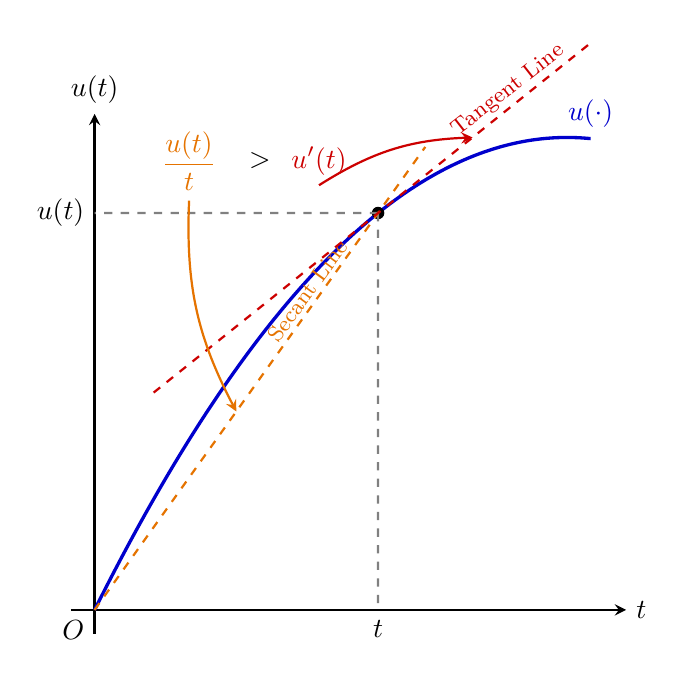
\begin{tikzpicture}[scale=1.5, thick, every node/.style={font=\sffamily}]
  % Axes
  \draw[->, >=stealth] (-0.2, 0) -- (4.5, 0) node[right] {$t$};
  \draw[->, >=stealth] (0, -0.2) -- (0, 4.2) node[above] {$u(t)$};
  \node[below left] at (0,0) {$O$};
  
  % Define a more curved concave function: u(t) = 2*t - 0.25*t^2
  % At t=2.4, u(2.4) = 3.36. 
  \draw[blue!80!black, very thick, domain=0:4.2, samples=100] plot (\x, {2*\x - 0.25*\x*\x}) node[above] {$u(\cdot)$};
  
  % Point t=2.4
  \coordinate (T) at (2.4, 3.36);
  \fill[black] (T) circle (1.5pt);
  \draw[dashed, gray] (T) -- (2.4, 0) node[below, text=black] {$t$};
  \draw[dashed, gray] (T) -- (0, 3.36) node[left, text=black] {$u(t)$};
  
  % Secant line (from origin through T)
  % Slope = 3.36 / 2.4 = 1.4
  \draw[orange!90!black, thick, dashed] (0, 0) -- (2.8, {1.4 * 2.8});
  \node[orange!90!black, font=\footnotesize, rotate=54] at (1.8, 2.7) {Secant Line};
  
  % Tangent line at T
  % Slope = u'(2.4) = 2 - 0.5*(2.4) = 0.8
  % Equation: y - 3.36 = 0.8(x - 2.4) => y = 0.8x + 1.44
  \draw[red!80!black, thick, dashed] (0.5, {0.8*0.5 + 1.44}) -- (4.2, {0.8*4.2 + 1.44});
  \node[red!80!black, font=\footnotesize, rotate=38] at (3.5, 4.4) {Tangent Line};
  
  % --- Visual indicator of inequality (Split into 3 nodes) ---
  % Left side: u(t)/t
  \node[text=orange!90!black, font=\normalsize] (left_expr) at (0.8, 3.8) {$\displaystyle\frac{u(t)}{t}$};
  % Middle: >
  \node[font=\normalsize] (gt) at (1.4, 3.8) {$>$};
  % Right side: u'(t)
  \node[text=red!80!black, font=\normalsize] (right_expr) at (1.9, 3.8) {$u'(t)$};
  
  % Arrows originating from the respective sides of the equation
  % Left side (orange) points to the secant line
  \draw[->, >=stealth, thick, orange!90!black, bend right=15] (left_expr.south) to (1.2, 1.68);
  
  % Right side (red) points to the tangent line
  \draw[->, >=stealth, thick, red!80!black, bend left=15] (right_expr.south) to (3.2, 4.0);
  
\end{tikzpicture}
\end{center}

\propp{Overbidding under Risk Aversion}{
  For any strictly positive valuation $x > 0$, a risk-averse bidder bids strictly higher than a risk-neutral bidder:
  \[
  \gamma(x) > \beta(x).
  \]
}{
  Note that a bidder with the lowest possible valuation ($x=0$) bids zero regardless of their risk attitude, so we have the boundary condition $\gamma(0) = \beta(0) = 0$.
  
  Suppose, for the sake of contradiction, that there exists some $x > 0$ where $\gamma(x) \le \beta(x)$. 
  Let $t = x - \gamma(x) > 0$. By the concavity property discussed above, $\frac{u(t)}{u'(t)} > t$, meaning:
  \[
  \frac{u(x-\gamma(x))}{u'(x-\gamma(x))} > x-\gamma(x) \ge x-\beta(x).
  \]
  Substituting this strict inequality into our differential equation for $\gamma'(x)$:
  \[
  \gamma'(x) = \frac{u(x-\gamma(x))}{u'(x-\gamma(x))} \cdot \frac{g(x)}{G(x)} > (x-\beta(x)) \cdot \frac{g(x)}{G(x)} = \beta'(x).
  \]
  This implies that at any point where $\gamma(x)$ is equal to or below $\beta(x)$, the slope of $\gamma$ is strictly steeper than the slope of $\beta$. 
  Since both functions start at the same origin ($\gamma(0) = \beta(0) = 0$), $\gamma$ must immediately rise above $\beta$. Furthermore, $\gamma$ can never cross $\beta$ from above, because at any intersection, $\gamma$ must be steeper. Thus, we conclude $\gamma(x) > \beta(x)$ for all $x > 0$.
}

\rmkb[The ``Insurance Premium" Intuition]{
  Why does a risk-averse bidder bid higher? In a First-Price Auction, a bidder faces a trade-off: bidding lower increases the profit \textit{if} they win, but increases the probability of losing and getting exactly zero. A risk-averse individual deeply dislikes the downside risk of losing the item. To protect themselves against this zero-payoff outcome, they are willing to sacrifice some potential profit by bidding more aggressively. In essence, the difference $\gamma(x) - \beta(x)$ is an \textbf{insurance premium} the bidder pays to increase their probability of winning.
}

Because risk aversion causes bidders to bid more aggressively in the FPA, while leaving the dominant strategy in the SPA unchanged, the expected payments in the FPA are strictly higher. Therefore, under risk aversion, {the First-Price Auction generates strictly higher expected revenue for the seller than the Second-Price Auction.}

